\documentclass[english,]{article}
\usepackage{lmodern}
\usepackage{amssymb,amsmath}
\usepackage{ifxetex,ifluatex}
\usepackage{fixltx2e} % provides \textsubscript
\ifnum 0\ifxetex 1\fi\ifluatex 1\fi=0 % if pdftex
  \usepackage[T1]{fontenc}
  \usepackage[utf8]{inputenc}
\else % if luatex or xelatex
  \ifxetex
    \usepackage{mathspec}
  \else
    \usepackage{fontspec}
  \fi
  \defaultfontfeatures{Ligatures=TeX,Scale=MatchLowercase}
\fi
% use upquote if available, for straight quotes in verbatim environments
\IfFileExists{upquote.sty}{\usepackage{upquote}}{}
% use microtype if available
\IfFileExists{microtype.sty}{%
\usepackage{microtype}
\UseMicrotypeSet[protrusion]{basicmath} % disable protrusion for tt fonts
}{}
\usepackage[margin=1in]{geometry}
\usepackage{hyperref}
\hypersetup{unicode=true,
            pdftitle={Trade Openness},
            pdfauthor={Winnie the Pooh},
            pdfborder={0 0 0},
            breaklinks=true}
\urlstyle{same}  % don't use monospace font for urls
\ifnum 0\ifxetex 1\fi\ifluatex 1\fi=0 % if pdftex
  \usepackage[shorthands=off,main=english]{babel}
\else
  \usepackage{polyglossia}
  \setmainlanguage[]{english}
\fi
\usepackage{graphicx,grffile}
\makeatletter
\def\maxwidth{\ifdim\Gin@nat@width>\linewidth\linewidth\else\Gin@nat@width\fi}
\def\maxheight{\ifdim\Gin@nat@height>\textheight\textheight\else\Gin@nat@height\fi}
\makeatother
% Scale images if necessary, so that they will not overflow the page
% margins by default, and it is still possible to overwrite the defaults
% using explicit options in \includegraphics[width, height, ...]{}
\setkeys{Gin}{width=\maxwidth,height=\maxheight,keepaspectratio}
\IfFileExists{parskip.sty}{%
\usepackage{parskip}
}{% else
\setlength{\parindent}{0pt}
\setlength{\parskip}{6pt plus 2pt minus 1pt}
}
\setlength{\emergencystretch}{3em}  % prevent overfull lines
\providecommand{\tightlist}{%
  \setlength{\itemsep}{0pt}\setlength{\parskip}{0pt}}
\setcounter{secnumdepth}{0}
% Redefines (sub)paragraphs to behave more like sections
\ifx\paragraph\undefined\else
\let\oldparagraph\paragraph
\renewcommand{\paragraph}[1]{\oldparagraph{#1}\mbox{}}
\fi
\ifx\subparagraph\undefined\else
\let\oldsubparagraph\subparagraph
\renewcommand{\subparagraph}[1]{\oldsubparagraph{#1}\mbox{}}
\fi

%%% Use protect on footnotes to avoid problems with footnotes in titles
\let\rmarkdownfootnote\footnote%
\def\footnote{\protect\rmarkdownfootnote}

%%% Change title format to be more compact
\usepackage{titling}

% Create subtitle command for use in maketitle
\newcommand{\subtitle}[1]{
  \posttitle{
    \begin{center}\large#1\end{center}
    }
}

\setlength{\droptitle}{-2em}
  \title{Trade Openness}
  \pretitle{\vspace{\droptitle}\centering\huge}
  \posttitle{\par}
  \author{Winnie the Pooh}
  \preauthor{\centering\large\emph}
  \postauthor{\par}
  \predate{\centering\large\emph}
  \postdate{\par}
  \date{5/25/2017}


\begin{document}
\maketitle

\subsection{Remarks:}\label{remarks}

\subsubsection{1. Use cloropleth maps with
caution}\label{use-cloropleth-maps-with-caution}

\begin{itemize}
\tightlist
\item
  One may easily manipulate color of a cloropleth map, see
\end{itemize}

\url{http://faculty.maxwell.syr.edu/mon2ier/e_reprints/StatSci%20Aug2005%20(Lying%20with%20Maps).pdf}

\begin{itemize}
\tightlist
\item
  Most cloropleth maps are just population maps
\end{itemize}

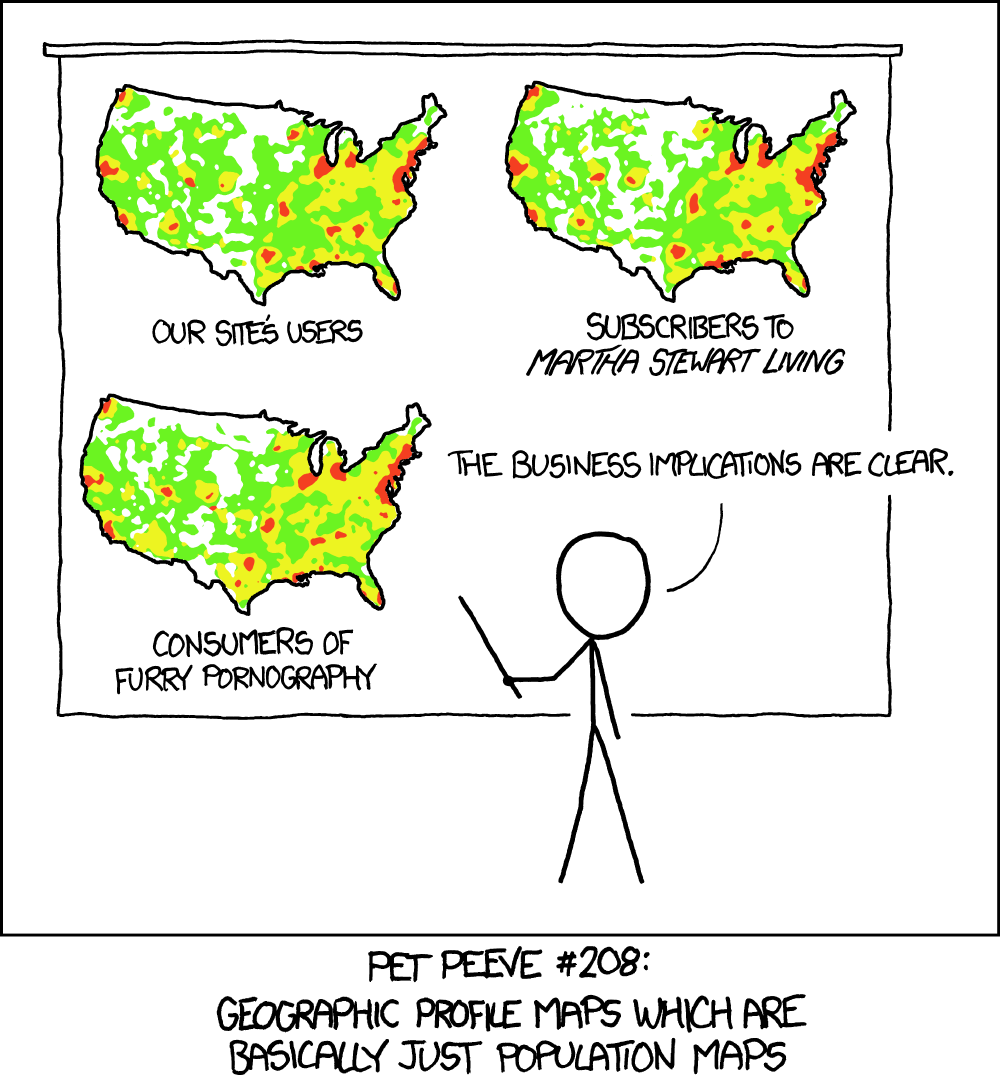
\includegraphics[width=8cm]{heatmap_2x.png}

\subsubsection{2. The use of instrumental variables is not equal to a
pure random
experiment}\label{the-use-of-instrumental-variables-is-not-equal-to-a-pure-random-experiment}

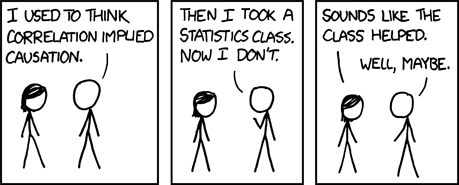
\includegraphics[width=8cm]{correlation.png}

\begin{itemize}
\tightlist
\item
  Try to find measure of African openness exogenous to Africa? Maybe
  sharp tax reduction in Europe or US?
\end{itemize}

\subsubsection{3. Compare import/export structure with Europe and US or
China}\label{compare-importexport-structure-with-europe-and-us-or-china}

\subsubsection{4. Structural changes in
fertility?}\label{structural-changes-in-fertility}

\begin{itemize}
\item
  Plot your time series!
\item
  Use mvtsplot: \url{http://www.biostat.jhsph.edu/~rpeng/RR/mvtsplot/}
\end{itemize}

\subsubsection{5. Small remarks}\label{small-remarks}

\begin{itemize}
\item
  Motivate why you omit Liberia
\item
  Less digits in table 1
\item
  Units of measure in Figure 2 and 3
\end{itemize}

\subsubsection{6. OLS and IV are just particular cases of
GMM}\label{ols-and-iv-are-just-particular-cases-of-gmm}

\subsubsection{7. Other variables:}\label{other-variables}

\begin{itemize}
\tightlist
\item
  religion
\item
  education
\item
  dictatorship, see
  \url{https://www.theguardian.com/world/2008/nov/27/south-africa-aids-mbeki}
\item
  health, AIDS (probably reverse causality?)
\end{itemize}

\subsubsection{8. Present more graphs and less
tables}\label{present-more-graphs-and-less-tables}

\begin{itemize}
\tightlist
\item
  Plot results of regression, Stata example,
  \url{http://www.stata.com/meeting/germany14/abstracts/materials/de14_jann.pdf}
\end{itemize}


\end{document}
